\chapter{Desarrollo}

A continuación se explicará la implementación detallada de cada uno de los componentes de la arquitectura. Puesto que el algoritmo a visualizar no es el contenido principal de este proyecto, se ha escogido uno cuya complejidad no sea excesiva. La elección ha sido el algoritmo \textit{Raft} \cite{10.5555/2643634.2643666} principalmente porque es muy adecuado para comprobar el funcionamiento de la interfaz. A diferencia de otros algoritmos que envían mensajes hasta alcanzar un objetivo, en \textit{Raft} se envían mensajes indefinidamente. Además de este aspecto, también es un algoritmo no demasiado complejo de comprender e implementar.

\section{Implementación del algoritmo \textit{Raft}}
\label{sec:raft}

Para la implementación del algoritmo \textit{Raft}, se ha escogido el lenguaje de programación \textit{Go} \cite{go}, que proporciona numerosas comodidades y ventajas a la hora de programar aplicaciones distribuidas. Por otra parte, la propuesta original de \textit{Raft} \cite{raft1} sugiere que la comunicación entre los nodos se implemente mediante llamadas a procedimientos remotos (RPC) puesto que se elimina la complejidad que supone enviar y recibir mensajes con \textit{sockets}. Sin embargo, en esta implementación, se ha diseñado la comunicación con mensajes tradicionales TCP. Además de que actualmente existen numerosas implementaciones del algoritmo empleando llamadas a procedimientos remotos \cite{raftetcd}, \cite{rafteliben}, la ventaja de los mensajes TCP es que es mucho más claro el proceso de envío y recepción de los mensajes.

Además de este aspecto, la implementación incluye la elección de líder completa y la replicación de \textit{log} parcial. La replicación no está completa puesto que esta implementación tiene como objetivo visualizar los mensajes relacionados con el algoritmo, y no el contenido de los \textit{logs} replicados. Por otra parte, la implementación está diseñada para interactuar con cada nodo mediante la entrada estándar del proceso. La función principal de la implementación (\textit{Main}) contiene la lógica necesaria para interactuar con los procesos en segundo plano que ejecutan el algoritmo. Las funcionalidades o comandos que incluye esta implementación son las siguientes:

\newpage

\begin{itemize}
\item\texttt{START}: Comenzar a ejecutar el algoritmo.
\item\texttt{STOP}: Detiene la ejecución del algoritmo.
\item\texttt{ADD}: Añade un nodo vecino. Se debe suministrar como parámetro la dirección válida del nodo vecino con formato \texttt{ip:puerto}.
\item\texttt{PEERS}: Imprime la lista de nodos vecinos.
\end{itemize}

A continuación se describe la implementación de cada uno de los componentes del algoritmo. La descripción simplificada de \textit{Raft} puede leerse en el Anexo, o en el artículo original \cite{raft1} (versión completa y detallada). Por otra parte, sólo se muestran partes del código simplificadas que no contienen control de errores.

Cuando un nodo comienza a ejecutar el algoritmo, comienzan a ejecutarse dos procesos secundarios. El primer proceso ejecuta la función \texttt{raft}, que contiene la mayoría del funcionamiento del algoritmo, mientras que el segundo ejecuta la función \texttt{listener}, que es la encargada de recibir mensajes del \textit{socket} TCP. La comunicación entre estas funciones se lleva a cabo mediante canales de \textit{Go} \cite{gochannels}, una de las mejores funcionalidades del lenguaje, que son similares a los \textit{pipes} de Linux. El proceso que ejecuta la función \texttt{raft} recibe mensajes de este canal, y en función del estado del nodo y otros factores, actúa de una manera u otra. Por otra parte la función \texttt{listener}, entre otras, envía mensajes al canal.

\subsection{Estado del algoritmo}

El estado del algoritmo se almacena en una estructura con los siguientes campos (se muestran únicamente los relacionados con la descripción del algoritmo):

\begin{lstlisting}[language=go]
type NodeStatus struct {
	peers              []NodeAddr     // Lista de nodos vecinos
	received_votes     int8           // Numero de votos recibidos en una eleccion
	voted_current_term bool           // Indica si se ha votado en el term acutal
	term               int            // Term actual
	log                []NodeLogEntry // Lista de entradas de log
	raftStatus         uint8          // Estado de raft: follower | candidate | leader
	electionTimeout    int64          // Tiempo de timeout para listener()
	leaderHeartbeat    int64          // Intervalo de tiempo entre mensajes para leaderHeartbeats()
	eventChan          chan Event     // Canal de comunicacion
}
\end{lstlisting}

\newpage

\subsection{Implementación de \texttt{listener}}

La implementación de la función \texttt{listener} es simple:

\begin{lstlisting}[language=go]
func listener(l *net.TCPListener, status *NodeStatus) {
	for {
		var timeout time.Time
		// Calcular en que instante habra timeout
		timeout = time.Now().Add(time.Millisecond * time.Duration(status.electionTimeout))
		// Establecer el timeout para el socket
		l.SetDeadline(timeout)

		// Esperar a una nueva conexion
		conn, err := l.Accept()
		if err != nil {
			if errors.Is(err, os.ErrDeadlineExceeded) {
				if status.raftStatus == candidate || status.raftStatus == follower {
					// Si se ha superado el timeout y el estado es candidate o follower
					// Escribir en el canal el evento de timeout
					status.eventChan <- Event{
						msg: NodeMsg{MsgType: followerTimeout},
					}
				} else {
					// Si es lider entonces este timeout no le afecta
				}
				continue
		}
		
		// Procesar la nueva conexion
		go responseHandler(conn, status)
	}
}
\end{lstlisting}

A esta función se le pasa como parámetro el estado del nodo, y el \textit{socket} por el que el nodo recibe mensajes. A modo de resumen, la funcionalidad se basa en esperar a recibir una nueva conexión en el \textit{socket} y procesar el mensaje con la función \texttt{responseHandler}, o bien enviar el evento de \textit{timeout} al canal de comunicación en el caso de que no se inicie una conexión en un tiempo determinado.

\subsection{Implementación de \texttt{responseHandler}}

La implementación de la función \texttt{responseHandler} es la siguiente:

\begin{lstlisting}[language=go]
func responseHandler(conn net.Conn, status *NodeStatus) {
	decoder := json.NewDecoder(conn)
	defer conn.Close()

	var msg NodeMsg
	decoder.Decode(&msg)
	
	status.eventChan <- Event{
		msg:    msg,
		sender: conn.RemoteAddr().(*net.TCPAddr).IP.String(),
	}
}
\end{lstlisting}

Esta función recibe del \textit{socket} un mensaje, lo \textit{deserializa} a un \texttt{struct} de \textit{Go} \cite{gostructs} y envía este objeto al canal.

\subsection{Implementación de \texttt{raft}}

La función que lee y procesa los mensajes del canal es \texttt{raft}, que implementa la mayoría de las funcionalidades del algoritmo.

\begin{lstlisting}[language=go]
func raft(wg *sync.WaitGroup, status *NodeStatus) {
	// Leer eventos del canal
	for event := range status.eventChan {
		switch event.msg.MsgType {
		// Si otro nodo ha comenzado una votacion		
		case requestVote:
			// Independientemente del estado, convertirse en follower si el term del mensaje es superior y si no se ha votado en el term actual
			if event.msg.Term > status.term && !status.voted_current_term {
				status.voted_current_term = true
				status.raftStatus = follower
				status.term = event.msg.Term
				go sendMsg(
					NodeMsg{MsgType: grantVote, Term: event.msg.Term},
					event.sender,
					event.msg.SenderPort,
				)
			}
		// Si es un mensaje de voto aceptado
		case grantVote:
			switch status.raftStatus {
			case follower:
				// No hace nada porque ya se termino la eleccion
			case candidate:
				// Mirar si es un voto a nuestra eleccion
				if event.msg.Term == status.term {
					status.received_votes++
					if int(status.received_votes) > (len(status.peers)+1)/2 {
						// Si se han recibido suficientes votos, convertirse en lider
						status.raftStatus = leader
						go leaderHeartbeats(status)
					}
				}
			case leader:
				// No hacer nada porque ya se ha conseguido ser lider
			}
		// Si es un mensaje con entradas de log
		case appendEntries:
			if event.msg.Term > status.term {
				// Si el term del mensaje es superior, convertirse en follower
				status.voted_current_term = false
				status.raftStatus = follower
				status.term = event.msg.Term
			}
		// Si es un evento de timeout
		case followerTimeout:
			switch status.raftStatus {
			case follower, candidate:
				// Comenzar eleccion si es follower o candidate
				go startElection(status)
			case leader:
				// Ignorar evento
			}
		}
	}
}
\end{lstlisting}

Como se puede observar, esta función altera el estado del algoritmo en función de los mensajes que recibe del canal y del estado en el que se encuentra:

\begin{itemize}
\item Cuando el mensaje que recibe es de tipo \texttt{requestVote}, significa que algún otro nodo ha iniciado una votación. En este escenario, el nodo se convertirá en seguidor si el nuevo \textit{term} es superior, y si no ha votado todavía en el \textit{term} actual.

\item En el caso de que el mensaje recibido sea de tipo \texttt{grantVote}, significa que el propio nodo ha iniciado una votación anteriormente, y algún otro nodo ha aceptado el voto. Si el nodo está en el estado \textit{follower}, se ignora la petición, puesto que la votación se ha terminado y no se ha conseguido el liderazgo. En el caso en el que el estado del nodo sea \textit{candidate}, hay que comprobar si el voto aceptado se corresponde con la votación actual. En el caso de que lo sea, el nodo se convierte en líder ejecutando la función \texttt{leaderHeartbeats} si ha recibido suficientes votos. En el caso de que el estado sea \textit{leader}, se ignora el mensaje, puesto que ya se ha conseguido el liderazgo.

\item En el caso de que se reciba un mensaje de tipo \texttt{appendEntries}, el nodo se convierte en seguidor si el \textit{term} del mensaje es superior al \textit{term} actual.

\item Si el tipo del mensaje es \texttt{followerTimeout}, significa que la función \texttt{listener} no ha recibido una nueva conexión en el tiempo del \textit{timeout}. Este escenario implica que el nodo inicie una votación (función \texttt{startElection}) en el caso de que sea seguidor o candidato.
\end{itemize}

\subsection{Implementación de \texttt{leaderHeartbeats}}

La función \texttt{leaderHeartbeats} se ejecuta cuando el estado del nodo es \textit{leader}. El objetivo es enviar periódicamente mensajes de tipo \texttt{appendEntries} a los nodos vecinos para que continúen en el estado \textit{follower}. Solamente termina cuando el estado del nodo deja de ser \textit{leader}. 

\begin{lstlisting}[language=go]
func leaderHeartbeats(status *NodeStatus) {
	for {
		if status.raftStatus != leader {
			return
		}

		msg := NodeMsg{
			MsgType:    appendEntries,
			Term:       status.term,
			Entries:    nil,
		}
		timeout := status.leaderHeartbeat
		
		// Enviar appendEntries a los vecinos
		for _, p := range status.peers {
			go sendMsg(msg, p.ip, p.port)
		}

		// Esperar para enviar la siguiente rafaga de appendEntries
		<-time.After(time.Duration(timeout) * time.Millisecond)
	}
}
\end{lstlisting}

\subsection{Implementación de \texttt{startElection}}

Por último, la función \texttt{startElection} es la encargada de enviar mensajes de tipo \texttt{requestVote} a los nodos vecinos cuando se inicia una nueva elección. 

\begin{lstlisting}[language=go]
func startElection(status *NodeStatus) {
	status.raftStatus = candidate
	status.term++
	status.received_votes = 1 // Votar por uno mismo

	msg := NodeMsg{
		MsgType:    requestVote,
		Term:       status.term,
		Entries:    nil,
	}

	for _, p := range status.peers {
		go sendMsg(msg, p.ip, p.port)
	}
}
\end{lstlisting}

\section{Implementación del proceso \textit{capturador}}

Como se describe en la sección~\ref{sec:arquitectura}, el proceso capturador debe capturar los mensajes de red que envía el nodo y reenviarlos al proceso manager. Además de esto, para permitir una comunicación bidireccional, debe ser capaz de interactuar con el proceso que ejecuta el algoritmo. Cabe destacar además que la comunicación entre los nodos del algoritmo no necesariamente debe ser a través de un mismo puerto siempre. En la implementación de \textit{Raft} de este proyecto, se reciben siempre desde el mismo puerto, pero se desconocen los puertos desde los que se envían los mensajes.

Actualmente existen múltiples librerías de programación de captura de mensajes de red, algunos ejemplos son \cite{libcap}, \cite{pyshark}, \cite{pypcap}. Sin embargo todas cuentan con una restricción, no se permite actualizar el filtro de paquetes de red dinámicamente. Esto es un inconveniente únicamente por la funcionalidad de añadir nodos vecinos durante la ejecución. Al añadir un nodo vecino, es necesario actualizar el filtro para incluir el puerto del nuevo nodo para capturar los mensajes enviados a ese nodo. Con las librerías existentes sería necesario detener la captura de mensajes, actualizar el filtro, y finalmente volver a comenzar la captura. Esta pausa en la escucha de mensajes de red puede suponer que no se capturen los mensajes en este intervalo de tiempo. Es por este motivo por el que se ha implementado un proceso capturador sin emplear librerías de este tipo.

El lenguaje de programación escogido para implementar este módulo es \textit{Python} \cite{python}, dado que permite implementar las funcionalidades necesarias de una forma sencilla comparado con otros lenguajes. La implementación se compone de dos partes, una con la función \texttt{sniffer} que captura los mensajes de red y los retransmite al proceso \textit{manager}, y otra con la funcionalidad relacionada con arrancar el nodo del algoritmo y comunicarse con él. Más adelante se detalla la implementación de estos módulos, comenzando por la función \texttt{sniffer}.

\subsection{Captura de mensajes}

Como se ha indicado anteriormente, las librerías existentes de captura de mensajes de red no permiten actualizar el filtro dinámicamente. Es por esto por lo que se ha implementado este módulo de captura personalizado. A continuación se muestra parte de la función \texttt{sniffer}.

\begin{lstlisting}[language=Python]
def sniffer():
    conn = socket.socket(socket.AF_PACKET, socket.SOCK_RAW, socket.ntohs(3))
    
    while True:
        # Get new packet
        raw_data, addr = conn.recvfrom(65535)
        
        # Get destination MAC, source MAC and ethernet protocol
        dest_mac, src_mac, eth_proto = struct.unpack('! 6s 6s H', raw_data[:14])
        eth_proto = socket.htons(eth_proto)
        data = raw_data[14:]

        # If packet is IPv4
        if eth_proto == 8:
            version_header_length = data[0]
            version = version_header_length >> 4
            header_length = (version_header_length & 15) * 4
            ttl, ip_proto, src_ip, target_ip = struct.unpack('! 8x B B 2x 4s 4s', data[:20])
            data = data[header_length:]

            # If TCP protocol
            if ip_proto == 6:
                src_port, dest_port, sequence, ack, offset_reserved_flags = struct.unpack('! H H L L H', data[:14])
                offset = (offset_reserved_flags >> 12) * 4
                flag_urg = (offset_reserved_flags & 32) >> 5
                flag_ack = (offset_reserved_flags & 16) >> 4
                flag_psh = (offset_reserved_flags & 8) >> 3
                flag_rst = (offset_reserved_flags & 4) >> 2
                flag_syn = (offset_reserved_flags & 2) >> 1
                flag_fin = offset_reserved_flags & 1
                data = data[offset:]

                # If packet has content for the application
                if flag_psh == 1 and dest_port in ports:
                    captured_msg = json.loads(data.decode())

                    captured_msg["SrcPort"] = captured_msg["SenderPort"]
                    captured_msg["SrcIp"] = "localhost"
                    captured_msg["DstPort"] = dest_port
                    captured_msg["DstIp"] = "localhost"

                    app_server.sendto(bytes(json.dumps(captured_msg), encoding='utf-8'), manager_addr)
\end{lstlisting}

Al principio se crea un \textit{socket} de red de tipo \texttt{SOCK\_RAW}, que recibe mensajes a nivel de protocolo \textit{ethernet}. Seguidamente se comienza un bucle infinito que ejecuta lo siguiente:

\begin{enumerate}
\item Guarda un nuevo mensaje en un buffer de máximo tamaño.
\item Obtiene las direcciones MAC origen y destino, y el protocolo \textit{ethernet}.
\item Comprueba si el paquete ha sido enviado desde el protocolo IPv4.
\item Extrae la información de la cabecera del paquete IP. Nótese que es necesario recurrir a operaciones de desplazamiento de bits dado que Python no permite indexar un byte a nivel de bit.
\item Comprueba si el paquete se ha enviado con el protocolo TCP.
\item Se extraen los datos de la cabecera TCP, entre los cuales se encuentran el \textit{flag} PSH, el puerto destino, el tamaño de la cabecera y el contenido del paquete.
\item Se comprueba si el puerto destino está en la lista de puertos de los nodos vecinos, y si el \textit{flag} PSH está a 1. Este \textit{flag} indica si el mensaje se envía al nivel de aplicación, es decir, indica si contiene datos de la aplicación.
\item Se envía un mensaje al proceso \textit{manager} con la información del mensaje capturado.
\end{enumerate}

Cabe destacar que la librería \texttt{socket} de \textit{Python} no incluye ninguna definición de sockets de este tipo para el sistema operativo \textit{Windows} \cite{pythonsocket}. Además de este aspecto, dado que el socket se ha declarado para recibir todos los mensajes \textit{ethernet}, es necesario ejecutar el código como \textit{superusuario}.

\subsection{Interacción con el proceso del algoritmo}

En cuanto a la gestión del proceso que ejecuta el algoritmo, se ha planteado la siguiente solución. Se ejecuta el proceso en un proceso hijo, de tal forma que se tiene acceso a distintos recursos, por ejemplo la entrada y la salida estándar. El código simplificado se muestra a continuación:

\begin{lstlisting}[language=Python]
process = subprocess.Popen('go run ./node/node.go', text=False, stdin=subprocess.PIPE, stdout=subprocess.PIPE, stderr=subprocess.PIPE, universal_newlines=False, shell=True)

while process.poll() is None:
    line = process.stdout.readline().decode()
    if line != "":
        print(">>> ", line, sep='', end='')

process.wait()
print("return_code:", process.returncode)
\end{lstlisting}

La primera línea inicializa la ejecución del algoritmo \textit{Raft}, indicando que se quiere acceder a la salida y entrada estándar. Seguidamente se comienza un bucle que imprime todos los mensajes que el proceso hijo muestra por la salida estándar. Este termina cuando el proceso hijo escribe en la salida estándar el carácter EOF (final de fichero). Finalmente se espera a que termine el proceso hijo para imprimir el valor de terminación.

\subsection{Interacción con el proceso \textit{manager}}

Por último, queda por explicar la forma en la que el proceso \textit{manager} se comunica con el proceso que ejecuta el algoritmo. Esto se consigue con la función \texttt{udp\_listener} (no confundir con la función \texttt{listener} del algoritmo \textit{Raft}).

\begin{lstlisting}[language=Python]
def udp_listener(process, node_port):
    with socket.socket(socket.AF_INET, socket.SOCK_DGRAM) as listener:
        listener.bind(("", 0)) # random port
        while True:
            msg_raw, addr = listener.recvfrom(2048)
            msg = json.loads(msg_raw.decode())
            final_msg = b'%s\n' % bytes(msg["args"], encoding='utf-8')
            
            process.stdin.write(final_msg)
            process.stdin.flush()
            
            if msg["type"] == "ADD":
                addPort(int(getPeerPort(final_msg)))
\end{lstlisting}

Como se puede observar, al comenzar se declara un socket de tipo UPD asignando un puerto aleatorio. En esta implementación se ha escogido el protocolo UDP para la comunicación con el proceso \textit{manager}. Se podría haber empleado cualquier otro tipo de protocolo de envío de mensajes de red. Sin embargo se ha escogido el protocolo UDP puesto que es un protocolo más rápido que TCP. La velocidad de transmisión de mensajes puede reducir la latencia en la visualización de mensajes en la interfaz.

El resto de la función consiste en un bucle infinito que recibe mensajes del proceso \textit{manager} y los escribe en la entrada estándar del proceso hijo (que ejecuta el algoritmo). Por otra parte, si el mensaje recibido de la interfaz indica que se quiere agregar un nuevo nodo, entonces se agrega el puerto a la lista de puertos que emplea el filtro de la función \texttt{sniffer}, descrita anteriormente.

\section{Descripción del cliente}

A continuación se describe la implementación del cliente. A modo de recordatorio la interfaz debe ser capaz de visualizar tanto los nodos del algoritmo como los mensajes que se envían en tiempo real, permitiendo al usuario interactuar de distintas formas. Para visualizar una red distribuida, sería necesario representar en un grafo las máquinas como nodos, y las conexiones como vértices. Las funcionalidades de representar estos elementos en pantalla y ofrecer la posibilidad arrastrar nodos para cambiar la distribución en pantalla, entre otras, son bastante complejas de implementar y no forman parte de los objetivos de este proyecto. Es por esto por lo que la elección del lenguaje de implementación se ha visto marcado por la existencia de alguna librería de programación que implemente estas funcionalidades. El lenguaje escogido es \textit{JavaScript} por los siguientes motivos:

\begin{itemize}
\item \textit{JavaScript} \cite{js} es el lenguaje que cuenta con más librerías a fecha de escritura \cite{libraries}, por tanto es más probable que contenga una que cumpla con los requisitos.

\item Además de ser el lenguaje con más librerías, es empleado extensamente en el desarrollo web, y por tanto está capacitado para implementar la lógica necesaria para controlar la interfaz de usuario.

\item Existen diferentes librerías que cumplen con los requisitos mencionados para representar grafos, algunos ejemplos son \cite{visjs}, \cite{gojs}, \cite{10.1093/bioinformatics/btv557}.
\end{itemize}

Por otra parte, la interfaz no ha sido implementará como una aplicación \textit{web} convencional, si no como una aplicación de \textit{electron}. Esto es imprescindible puesto que desde la versión \textit{web} de \textit{JavaScript} no es posible enviar mensajes de red, por motivos de seguridad. \textit{Electron}\cite{electron} es un \textit{framework} que permite desarrollar aplicaciones de escritorio multiplataforma empleando recursos de desarrollo \textit{web}, por ejemplo \textit{HTML}, \textit{CSS} y \textit{JavaScript}.

En cuanto a la librería de visualización de grafos, se ha escogido \textit{Vis.js} \cite{visjs}, puesto que además de ser gratuita y de código abierto, permite visualizar animaciones que recorren los vértices del grafo. Estas animaciones se emplean para representar el tráfico de red entre los nodos del algoritmo. En lo restante de este apartado se detalla el funcionamiento de los botones de la interfaz, y cómo interactúa el cliente con el proceso \textit{capturador}. La interfaz final de la aplicación puede apreciarse en la imagen de la figura~\ref{fig:dave1}.

%\begin{figure}[h]
%  \centering
%  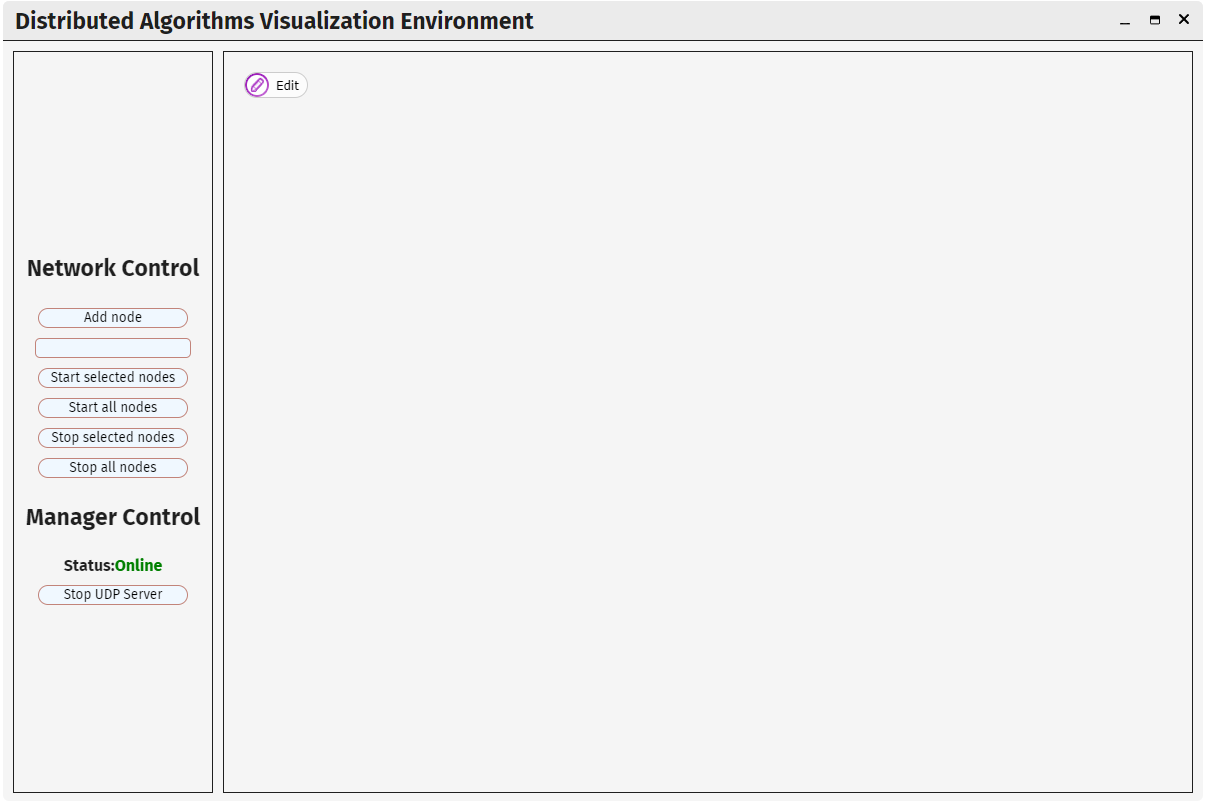
\includegraphics[width=0.9\linewidth]{imagenes/dave1}
%  \caption{Captura de pantalla de la interfaz}
%  \label{fig:dave1}
%\end{figure}
{
\centering
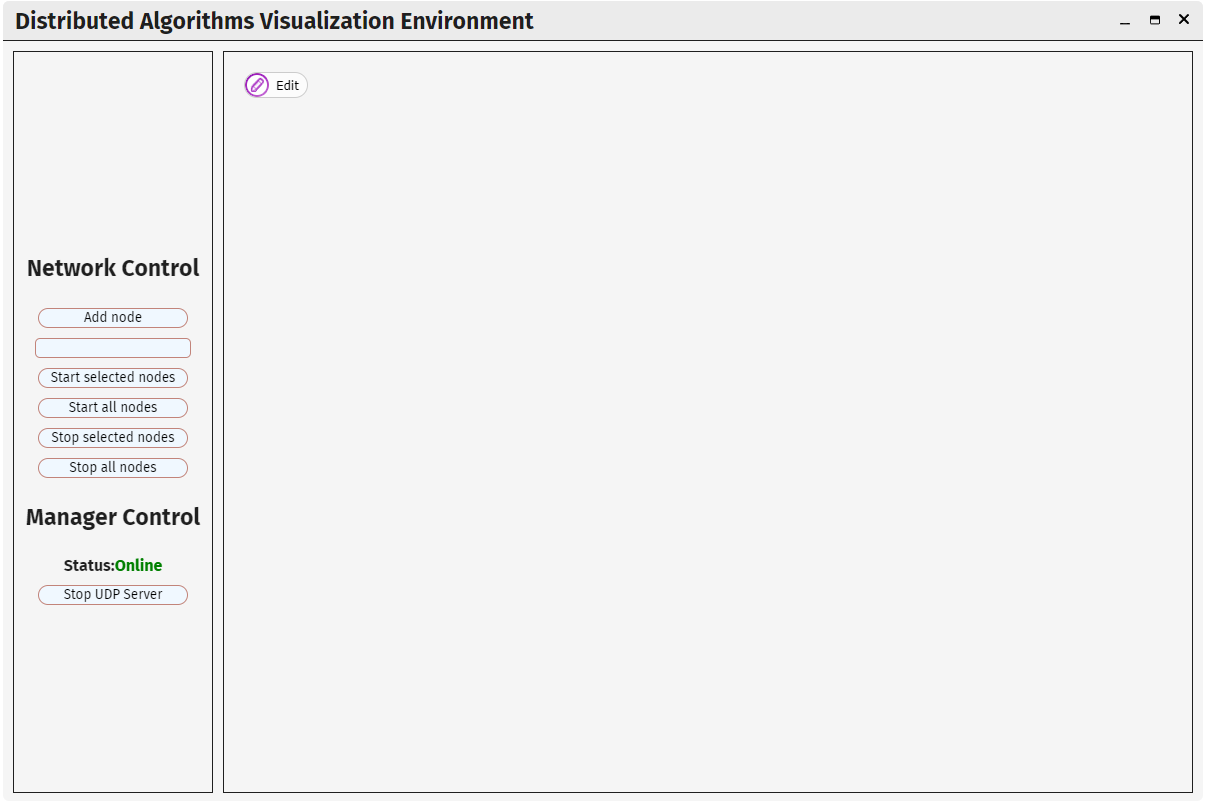
\includegraphics[width=0.9\linewidth]{imagenes/dave1}
\captionof{figure}{Captura de pantalla de la interfaz}
\label{fig:dave1}
}

Como se puede observar, en la parte izquierda de la pantalla se localizan los controles, y en la derecha el marco donde se dibujará el grafo del algoritmo. Los controles se dividen en dos partes, una que controla los nodos, y otra que controla el proceso \textit{manager}. Como se ha descrito anteriormente, el proceso capturador recibe mensajes a través de un \textit{socket} de red, al mismo tiempo que los retransmite al proceso que ejecuta el algoritmo. Estos mensajes, se envían desde la interfaz pulsando alguno de los siguientes botones:

\newpage

\begin{itemize}
\item Botones ''\textit{Start selected nodes}'' y ''\textit{Start all nodes}'': comienzan la ejecución de los nodos seleccionados o de todos los nodos, respectivamente. Se envía un mensaje correspondiente al comando \texttt{START}, que se describió durante la sección~\ref{sec:raft}.

\item Botones ''\textit{Stop selected nodes}'' y ''\textit{Stop all nodes}'': tienen el mismo comportamiento que el último, excepto que detienen la ejecución de uno o más nodos enviando el mensaje correspondiente al comando \texttt{START}.

\item Botón ''\textit{Add node}'': añade un nodo a la visualización. Se debe suministrar la dirección de nodo a añadir.
\end{itemize}

Por la parte de la sección de control del proceso \textit{manager}, se puede detener y arrancar el proceso. Pudiendo observar el estado de este en la parte superior al botón. La interfaz es completamente ''\textit{responsive}'' como se dice en el ámbito del desarrollo web, lo cual significa que el tamaño de los elementos en la pantalla se adapta automáticamente para mostrar todo el contenido cuando se cambia de tamaño la ventana.

Más adelante, en el siguiente apartado, se explica la funcionalidad del proceso \textit{manager} y cómo interactúa con la visualización para mostrar los eventos que se producen en el algoritmo. 

\section{Implementación del \textit{manager}}

Como se ha descrito anteriormente, el proceso \textit{manager} debe contener toda la funcionalidad relacionada con recibir mensajes de todos los procesos capturadores, y modificar la visualización de acuerdo con el origen, destino y contenido de estos. Puesto que es un proceso que debe interactuar con la representación de la red que se visualiza, es necesario que sea implementado junto con la interfaz para tener acceso a las variables del programa necesarias.

En \textit{electron} se puede implementar fácilmente un proceso servidor con el módulo \texttt{dgram}, que permite crear y manejar \textit{sockets} UDP. La implementación básica de un servidor de este tipo se muestra a continuación:

\begin{lstlisting}[language=JavaScript]
const dgram = require('dgram');
var server;

function start_server() {
    server = dgram.createSocket('udp4');

    server.on('error', function(err) {
        // Error
    });

    server.on('message', function(msg, rinfo) {
    	// Procesar mensaje
    });

    server.on('listening', function() {
        // Socket listo para recibir mensajes
    });

    server.on('close', function() {
        // El socket se ha cerrado
    });
    
    // Asignar un puerto de escucha
    server.bind(3333);
}
\end{lstlisting}

Como se puede observar, la implementación en \textit{JavaScript} de un servidor UDP es sencilla. Por cada evento del \textit{socket} (\texttt{error}, \texttt{message}, \texttt{listening} y \texttt{close}) se asocia una función que se ejecuta cada vez que el evento se produce. En el caso de este Trabajo de Fin de Grado, la más importante claramente es la función asociada al evento \texttt{message}, que se ejecuta cada vez que se recibe un mensaje. Esta función debe ser capaz de actualizar la interfaz de acuerdo con el contenido del mensaje. A continuación se muestra parte de la implementación final del servidor:

\begin{lstlisting}[language=JavaScript]
function start_server() {
    server = dgram.createSocket('udp4');

    server.on('error', function(err) {
        print('start_server', err.stack)
        server.close();
    });

    server.on('message', function(msg, rinfo) {
        print('start_server', `msg from ${rinfo.address}:${rinfo.port}\n${msg}`);
        var parsed_msg = JSON.parse(msg);
        var e = `${parsed_msg.SrcIp}:${parsed_msg.SrcPort}_${parsed_msg.DstIp}:${parsed_msg.DstPort}`

        // Animate message
        console.log(`Edge: ${e}`);
        network.animateTraffic([{
            edge: e,
            trafficSize: 5,
        }]);
        
        // Update node labels
        var aux_id = `${parsed_msg.SrcIp}:${parsed_msg.SrcPort}`;
        network_nodes.update([{
            id: aux_id,
            label: formatLabel(
                parsed_msg.SrcIp,
                nodes[aux_id].port,
                parsed_msg.SrcPort,
                parsed_msg.Term
            ),
        }]);
    });

    server.on('listening', function() {
        const address = server.address();
        print('start_server', `listening on ${address.address}:${address.port}`);
    });

    server.on('close', function() {
        print('start_server', 'Closed server');
    });

    server.bind(3333);
}
\end{lstlisting}

En la implementación del cliente se emplean varias funciones auxiliares. Una de ellas es \texttt{print}, que imprime mensajes de log en la consola formateados para su lectura fácil. Recibe como primer parámetro la función que la llama, y como segundo el mensaje. De esta manera es posible determinar el origen de los mensajes de log. Por otra parte se emplea la función \texttt{formatLabel}, que formatea varios parámetros a mostrar en la interfaz de cada nodo.

Como se puede observar la función asociada al evento \texttt{message} averigua, según la información sobre la conexión proporcionada por el \textit{socket}, el vértice del grafo que se corresponde con la conexión entre el nodo origen. Además de esto, también obtiene los identificadores de ambos nodos implicados en la comunicación.

La gestión de animaciones de la interfaz que representan los mensajes se lleva a cabo con la función \texttt{animateTraffic}, incluida con la librería de visualización de grafos. Admite como parámetro una lista de vértices en los que mostrar una animación, pero en el caso de este proyecto se indica sólo uno dado que se visualiza únicamente un mensaje por cada evento \texttt{message}.

\section{Caso de uso}

En este apartado se demuestra la funcionalidad completa de la aplicación con un algoritmo concreto: \textit{Raft}. Cabe destacar que los pasos mostrados a continuación son únicamente un ejemplo concreto. Como es lógico, no es posible incluir tantas imágenes como combinaciones posibles de acciones del usuario.

En primer lugar, es necesario ejecutar por una parte la aplicación de escritorio y por otra todas las instancias que se deseen del proceso capturador. Una vez inicializadas se introduce en el campo asociado con el botón ''\textit{Add node}'' de la interfaz, una a una cada dirección de cada instancia. El proceso capturador muestra convenientemente, por la salida estándar, la dirección del nodo con el formato adecuado para que el usuario únicamente tenga que copiar y pegar la información, sin necesidad de escribir manualmente. El resultado de insertar varios nodos en el sistema de visualización es se puede apreciar en la captura de pantalla de la figura~\ref{fig:ui1}.

\newpage

%\begin{figure}[h]
%  \centering
%  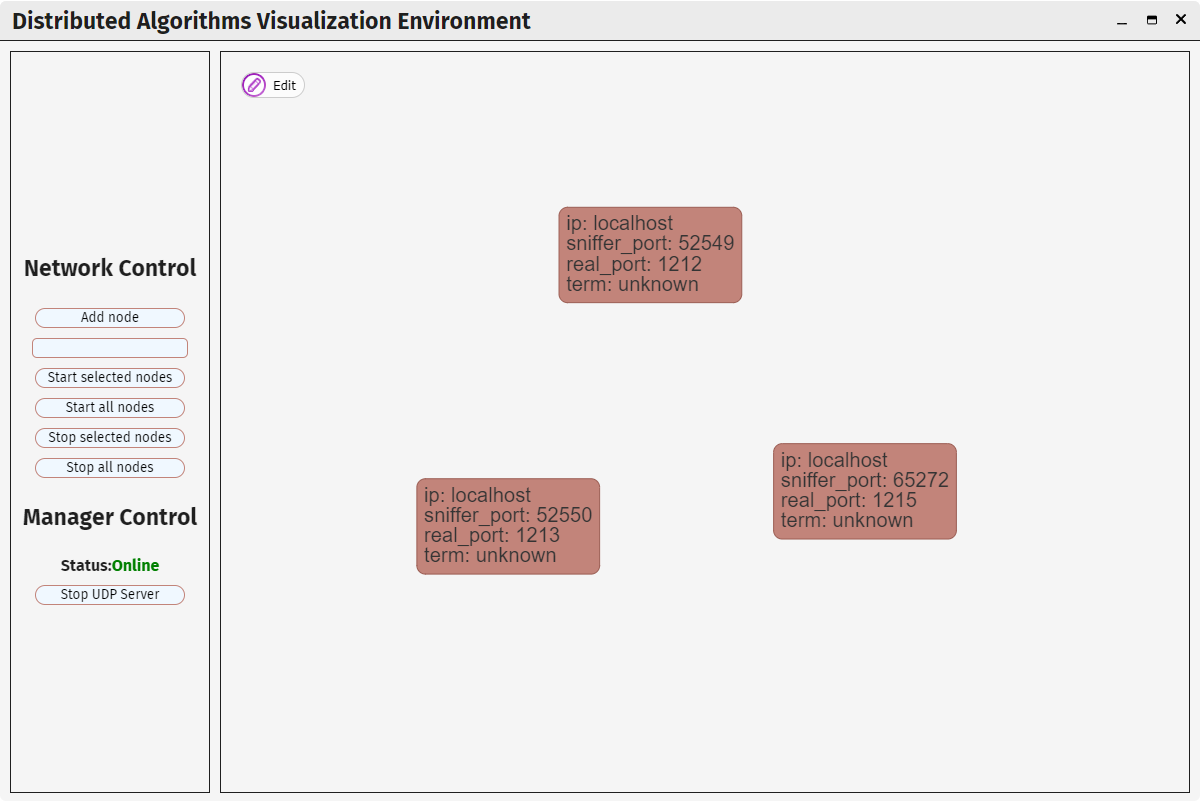
\includegraphics[width=0.9\linewidth]{imagenes/ui1}
%  \caption{Resultado de añadir varios nodos en la visualización}
%  \label{fig:ui1}
%\end{figure}

{
\centering
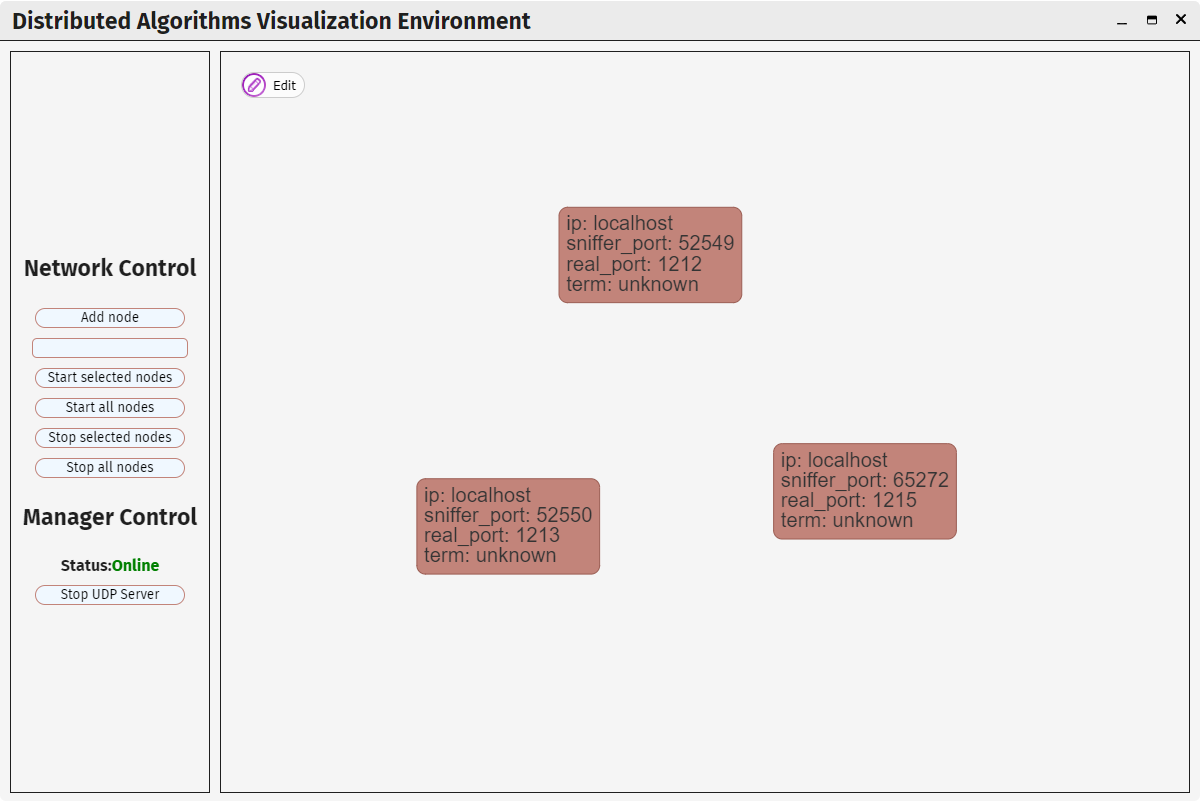
\includegraphics[width=0.9\linewidth]{imagenes/ui1}
\captionof{figure}{Resultado de añadir varios nodos en la visualización}
\label{fig:ui1}
}

Los contenidos visualizados de cada nodo son los siguientes: puerto del algoritmo, puerto del proceso capturador, dirección IP del nodo, y \textit{term} actual. Como se puede observar, se desconoce el \textit{term} de cada nodo. Esto se debe a que la visualización del algoritmo únicamente conoce el estado a partir del contenido de los mensajes que captura el proceso capturador. Puesto que todavía no se han enviado mensajes, esta información es desconocida por el momento.

En las figuras~\ref{fig:ui2},~\ref{fig:ui3} y~\ref{fig:ui4} se muestra el procedimiento seguido para añadir una nueva conexión. En primer lugar, se pulsa en el botón de edición para acceder al menú de conexiones, esto se puede observar en la figura~\ref{fig:ui2}. Seguidamente se pulsa el botón ''\textit{Add Connection}''. A continuación se pulsa en un nodo y, manteniendo la pulsación, se arrastra el puntero hasta otro nodo donde se suelta (Figura~\ref{fig:ui3}). El resultado son dos vértices entre ambos nodos, cada uno simboliza la conexión en un sentido. El resultado final de este paso se muestra en la figura~\ref{fig:ui4}. A continuación se sigue el mismo procedimiento para añadir las conexiones restantes que se deseen. Un ejemplo de configuración final se puede apreciar en la figura~\ref{fig:ui5}.

\newpage

%\begin{figure}[p]
%  \centering
%  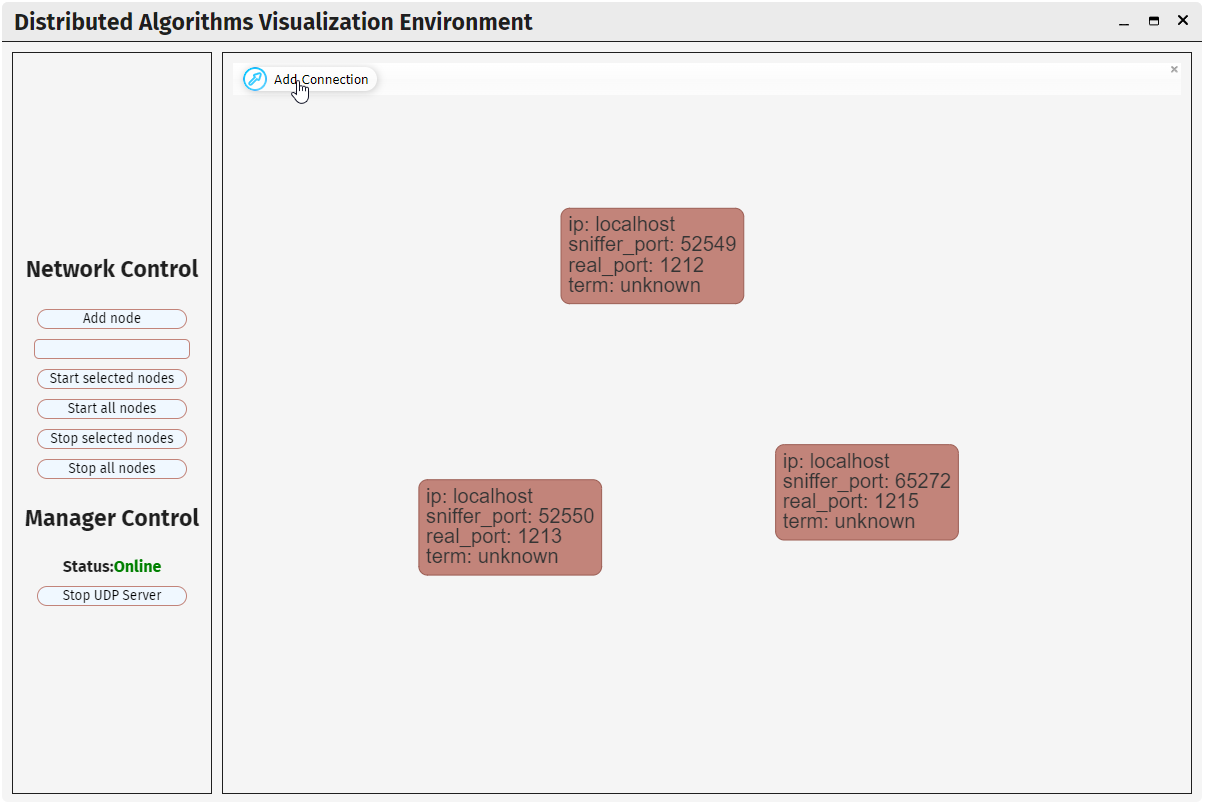
\includegraphics[width=0.9\linewidth]{imagenes/ui2}
%  \caption{Menú de conexiones}
%  \label{fig:ui2}
%\end{figure}
{
\centering
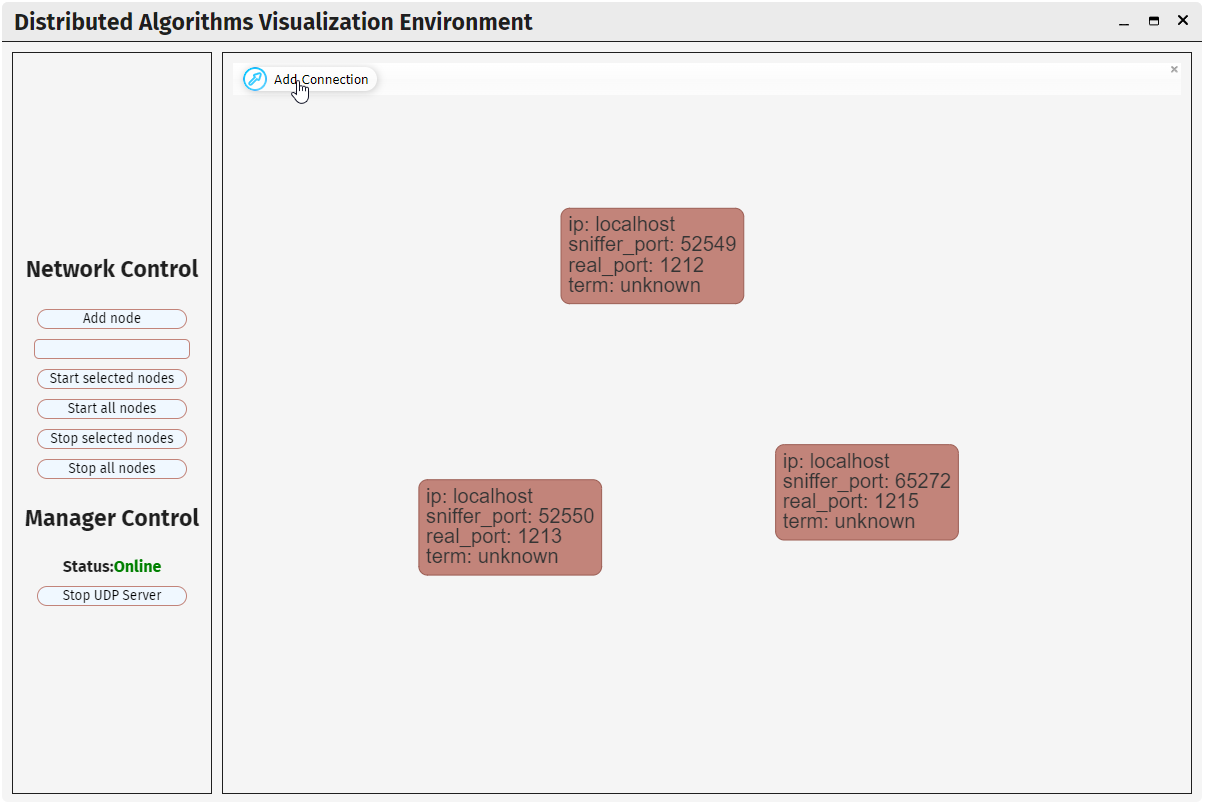
\includegraphics[width=0.9\linewidth]{imagenes/ui2}
\captionof{figure}{Menú de conexiones}
\label{fig:ui2}
}

%\begin{figure}[p]
%  \centering
%  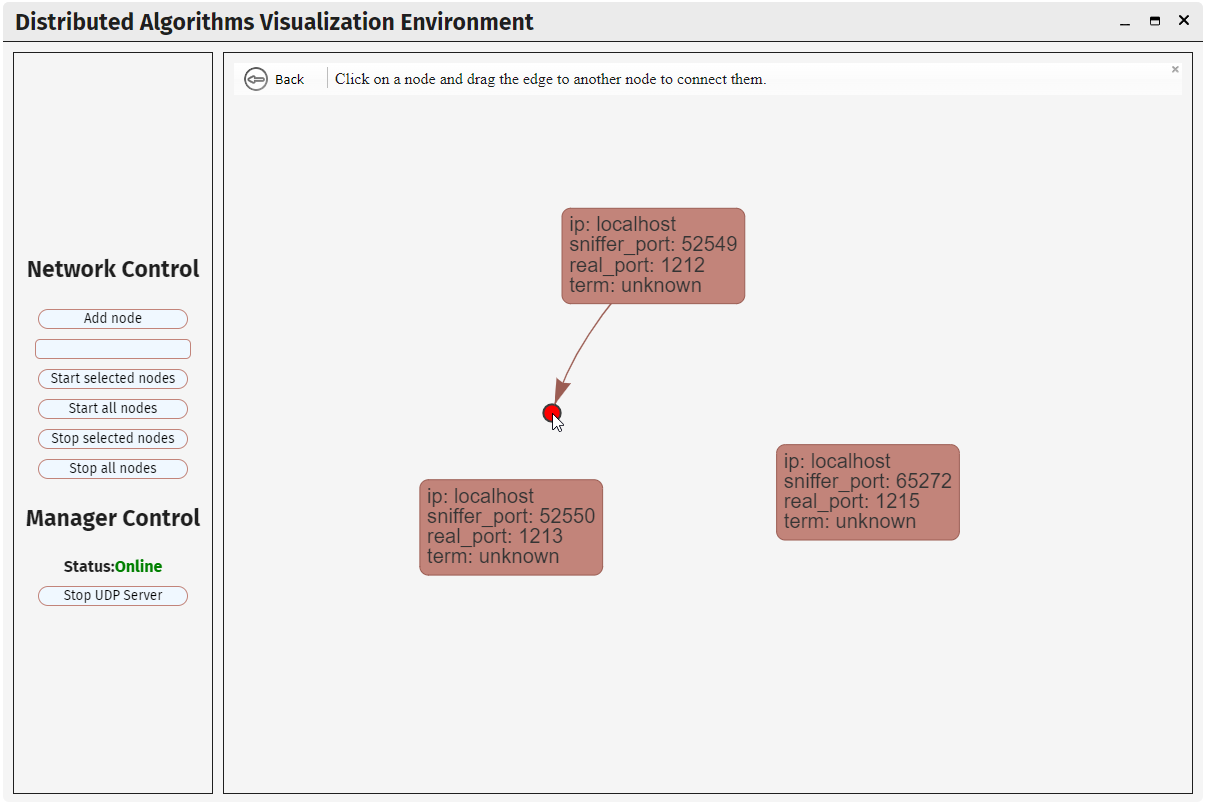
\includegraphics[width=0.9\linewidth]{imagenes/ui3}
%  \caption{Proceso de crear una nueva conexión}
%  \label{fig:ui3}
%\end{figure}
{
\centering
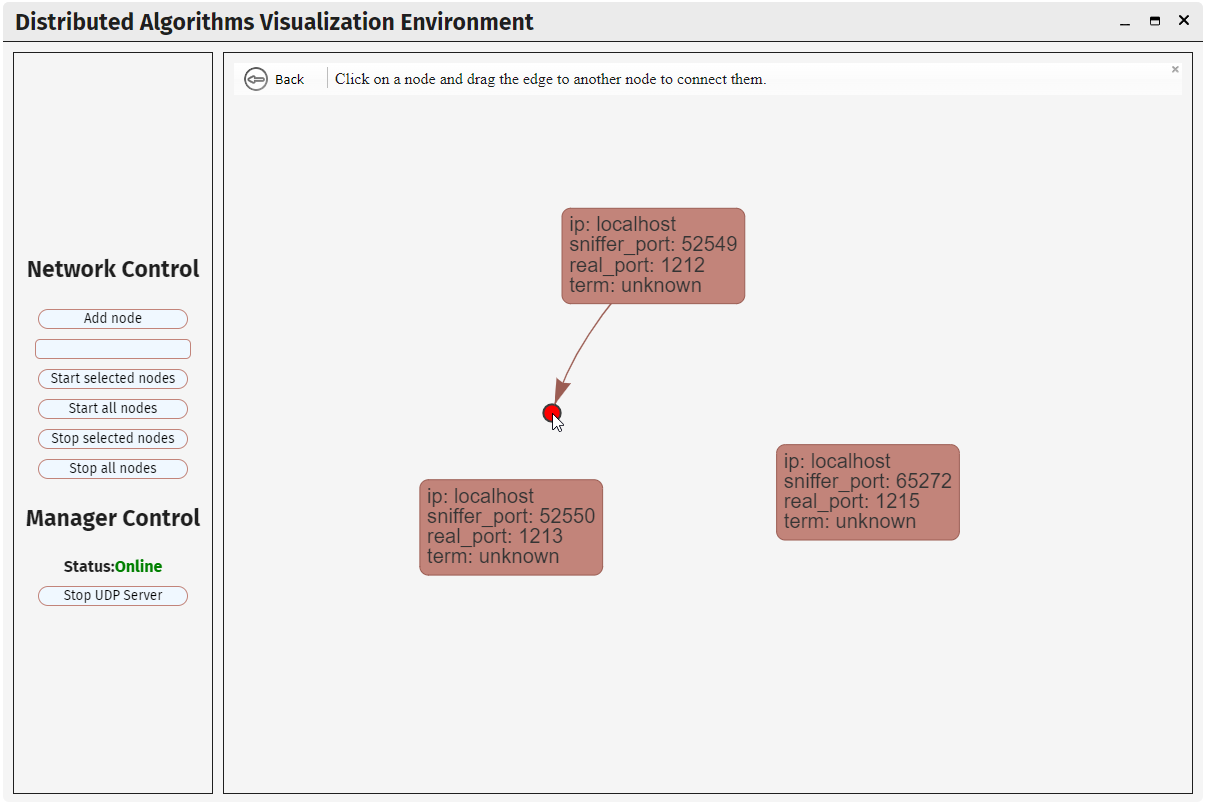
\includegraphics[width=0.9\linewidth]{imagenes/ui3}
\captionof{figure}{Proceso de crear una nueva conexión}
\label{fig:ui3}
}

\newpage

%\begin{figure}[p]
%  \centering
%  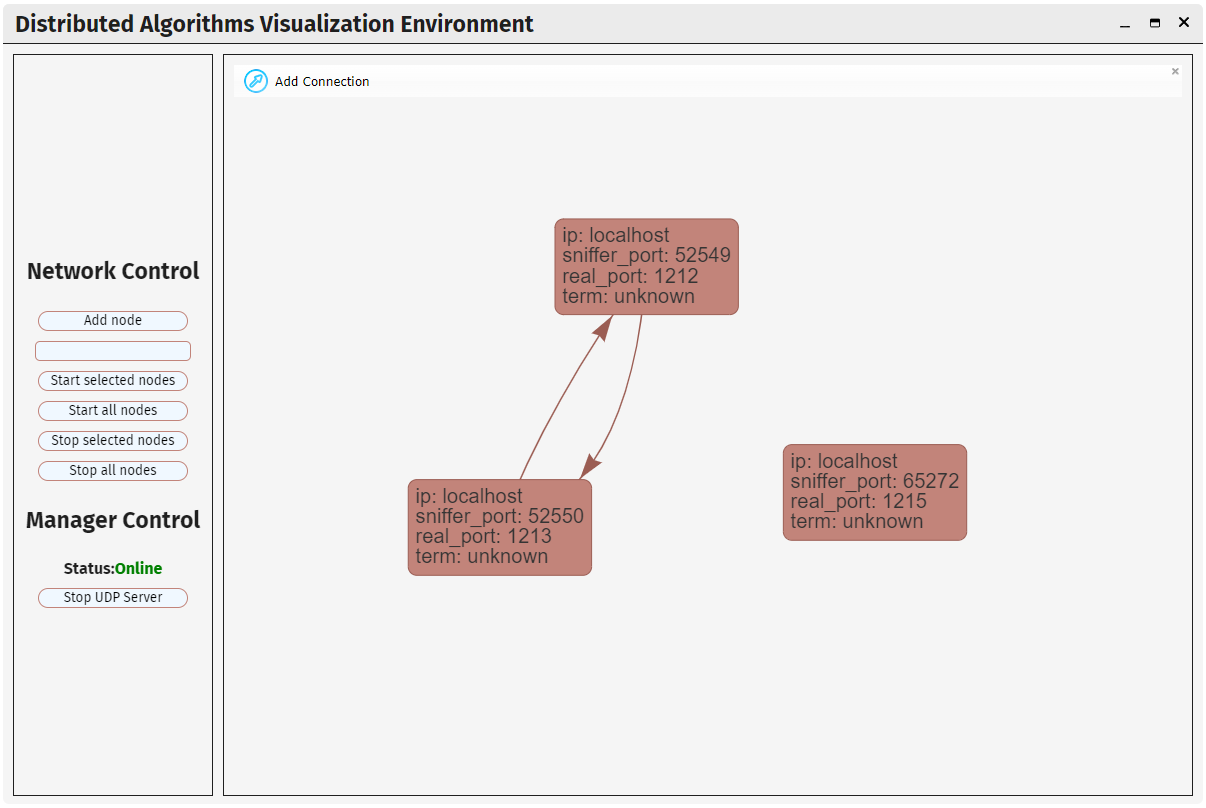
\includegraphics[width=0.9\linewidth]{imagenes/ui4}
%  \caption{Resultado de añadir una nueva conexión}
%  \label{fig:ui4}
%\end{figure}
{
\centering
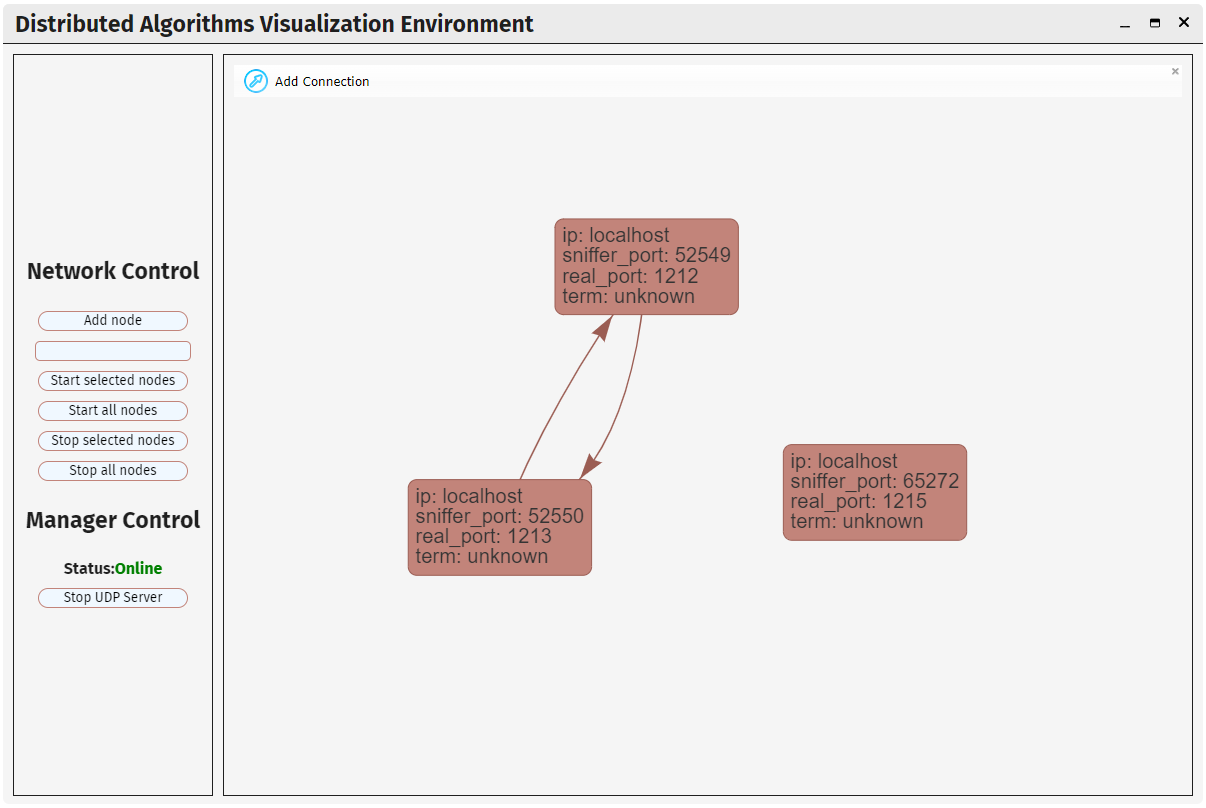
\includegraphics[width=0.9\linewidth]{imagenes/ui4}
\captionof{figure}{Resultado de añadir una nueva conexión}
\label{fig:ui4}
}

%\begin{figure}[p]
%  \centering
%  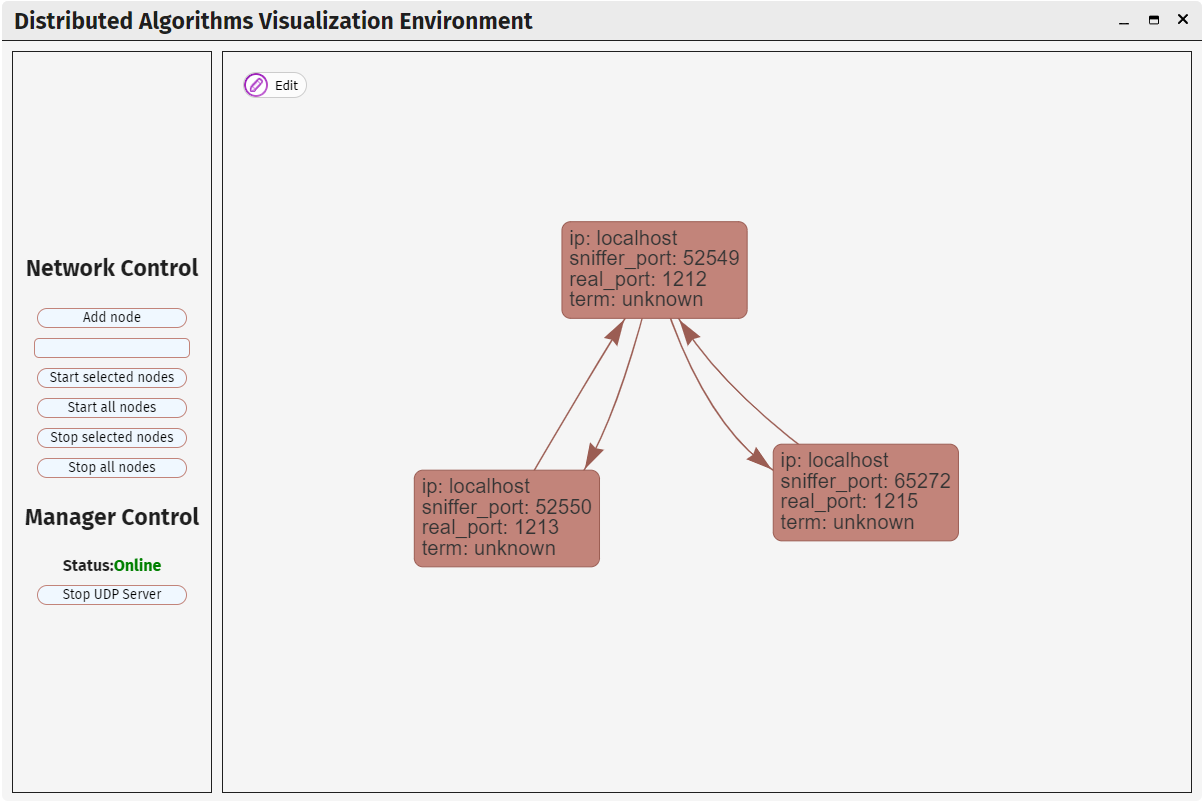
\includegraphics[width=0.9\linewidth]{imagenes/ui5}
%  \caption{Resultado de añadir todas las conexiones}
%  \label{fig:ui5}
%\end{figure}
{
\centering
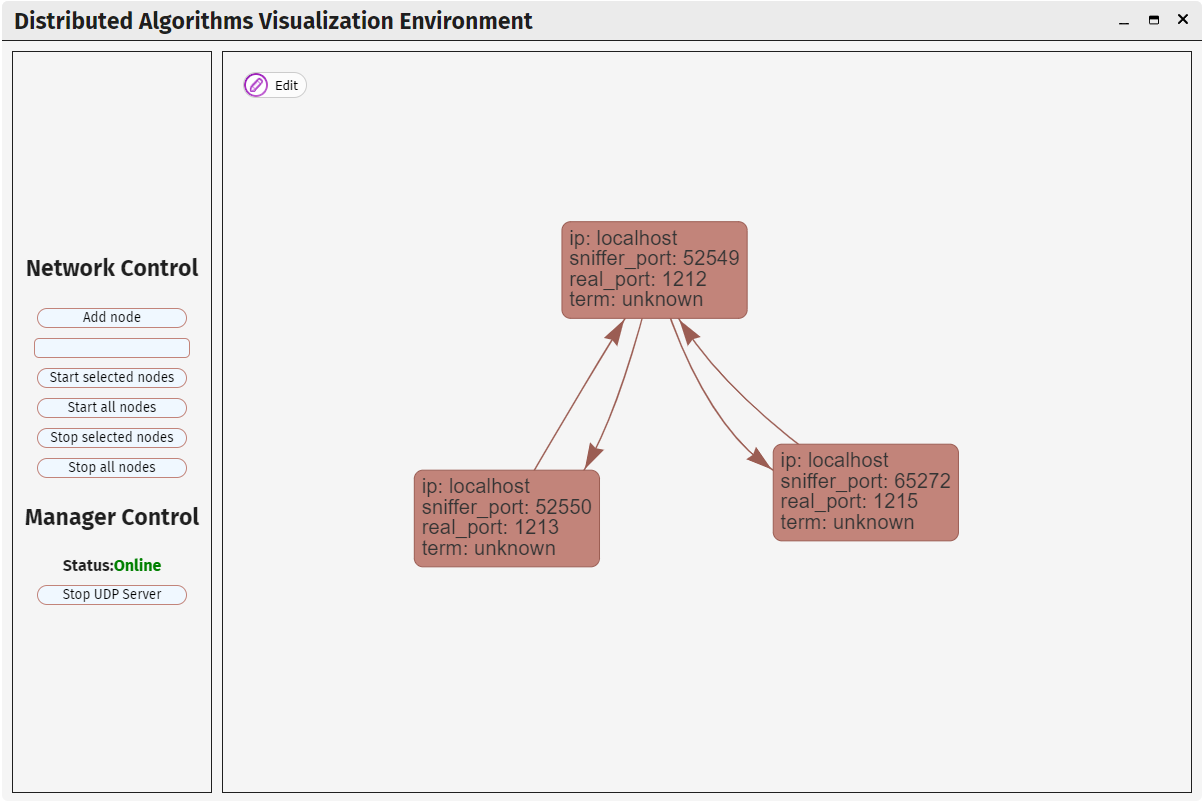
\includegraphics[width=0.9\linewidth]{imagenes/ui5}
\captionof{figure}{Resultado de añadir todas las conexiones}
\label{fig:ui5}
}

\newpage

Ahora que se han añadido los nodos y conexiones deseados, se puede proceder a iniciar la ejecución de cada uno de los nodos. Para ello se pulsará sobre un nodo para seleccionarlo, y posteriormente se pulsará el botón ''\textit{Start selected nodes}''. Seguidamente se seleccionarán los nodos restantes y se pulsará el mismo botón de nuevo. Esto provocará que el primer nodo sea líder puesto que comenzará la ejecución antes que los demás. A partir de este momento, los mensajes entre nodos se mostrarán como círculos azules recorriendo los vértices. Como es lógico, en la imagen no se muestra la animación. Cabe destacar que el campo \textit{term} cuyo valor antes era desconocido, ahora se conoce puesto que se extrae de los mensajes. El resultado final se puede apreciar en la figura~\ref{fig:ui6}.

%\begin{figure}[p]
%  \centering
%  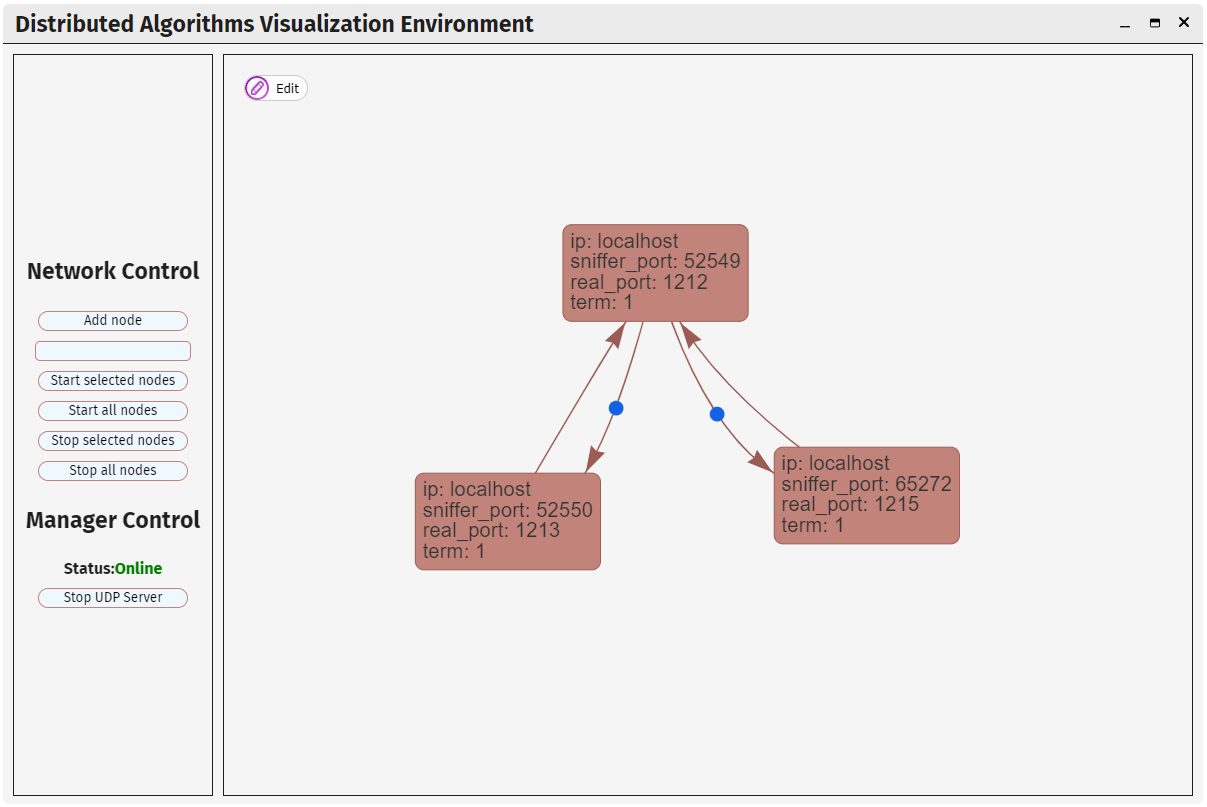
\includegraphics[width=0.9\linewidth]{imagenes/ui6}
%  \caption{Visualización del tránsito de mensajes}
%  \label{fig:ui6}
%\end{figure}
{
\centering
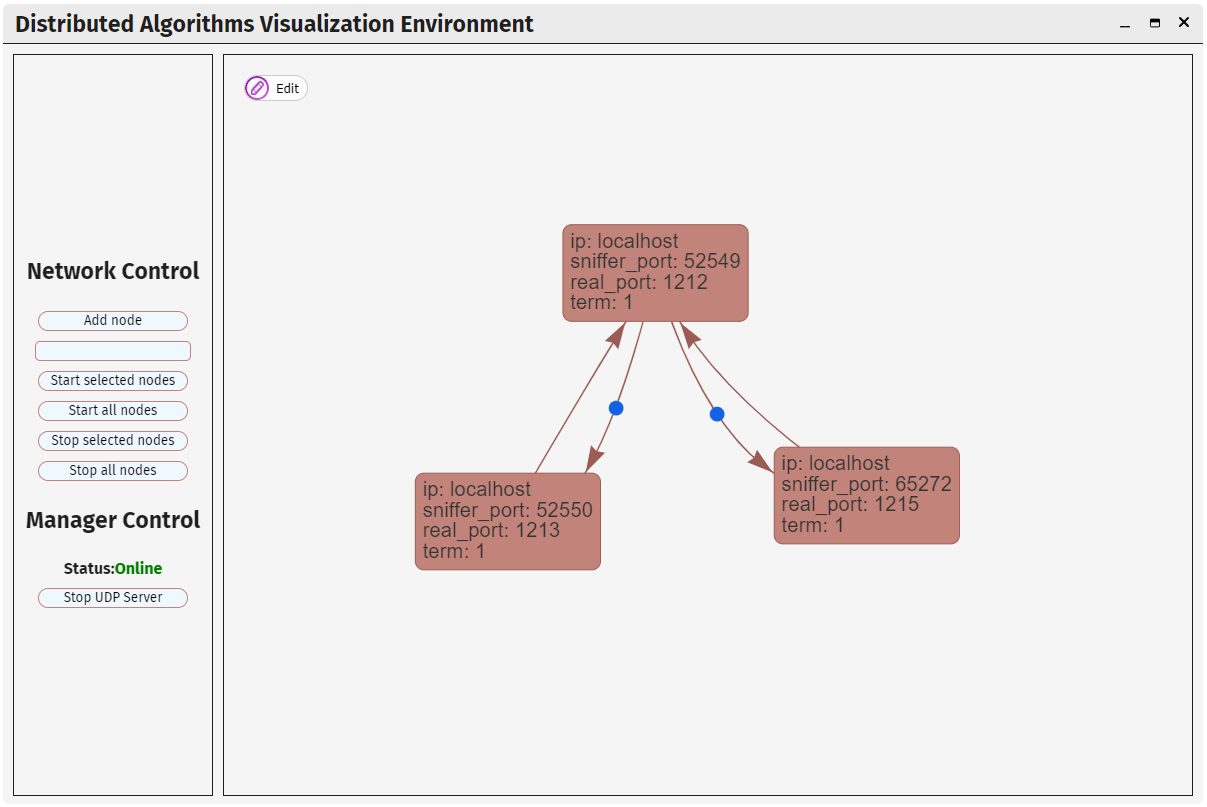
\includegraphics[width=0.9\linewidth]{imagenes/ui6}
\captionof{figure}{Visualización del tránsito de mensajes}
\label{fig:ui6}
}

Cabe destacar que no es necesario añadir todos los nodos y las conexiones antes de arrancar la ejecución de estos. Se pueden añadir sin problema durante la ejecución. Un ejemplo de esto se muestra en las figuras~\ref{fig:ui7} y~\ref{fig:ui8}, donde se añade otro nodo y se conecta a uno de los nodos existentes.

\newpage

%\begin{figure}[p]
%  \centering
%  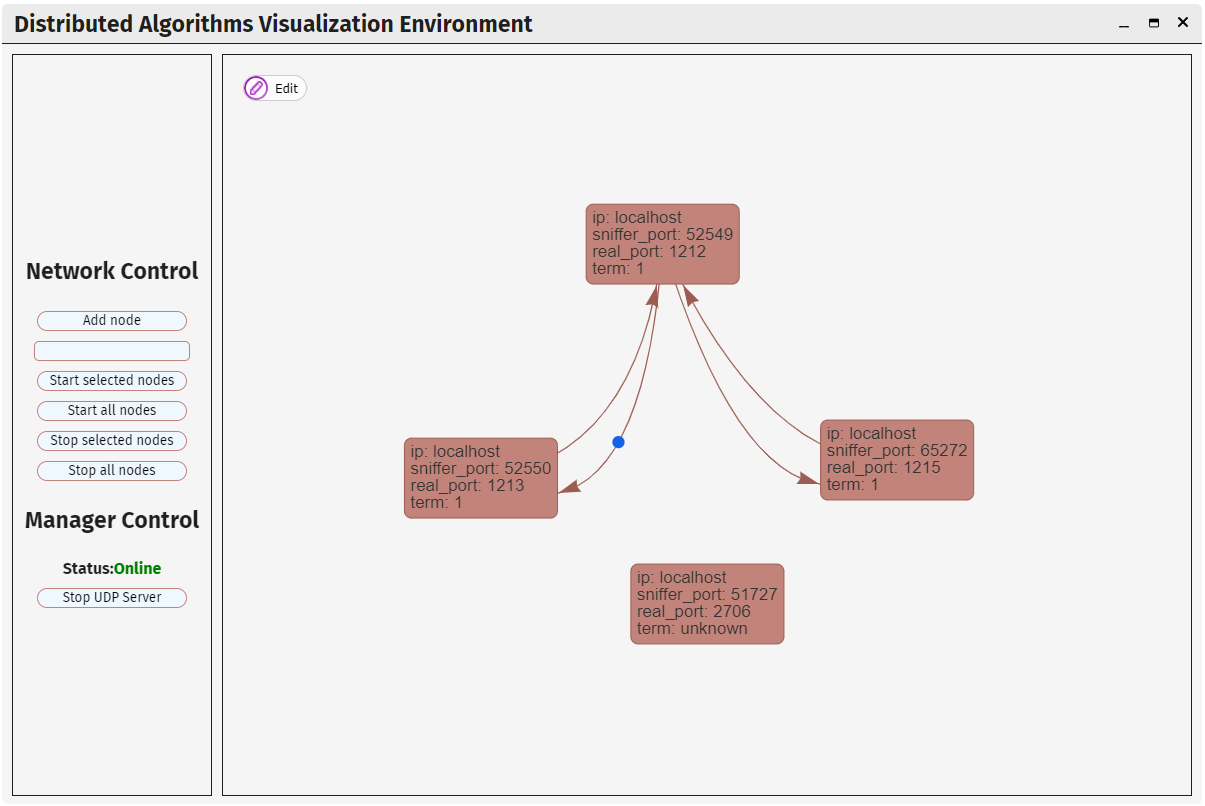
\includegraphics[width=0.9\linewidth]{imagenes/ui7}
%  \caption{Añadir nodo nuevo durante la ejecución de otros nodos}
%  \label{fig:ui7}
%\end{figure}
{
\centering
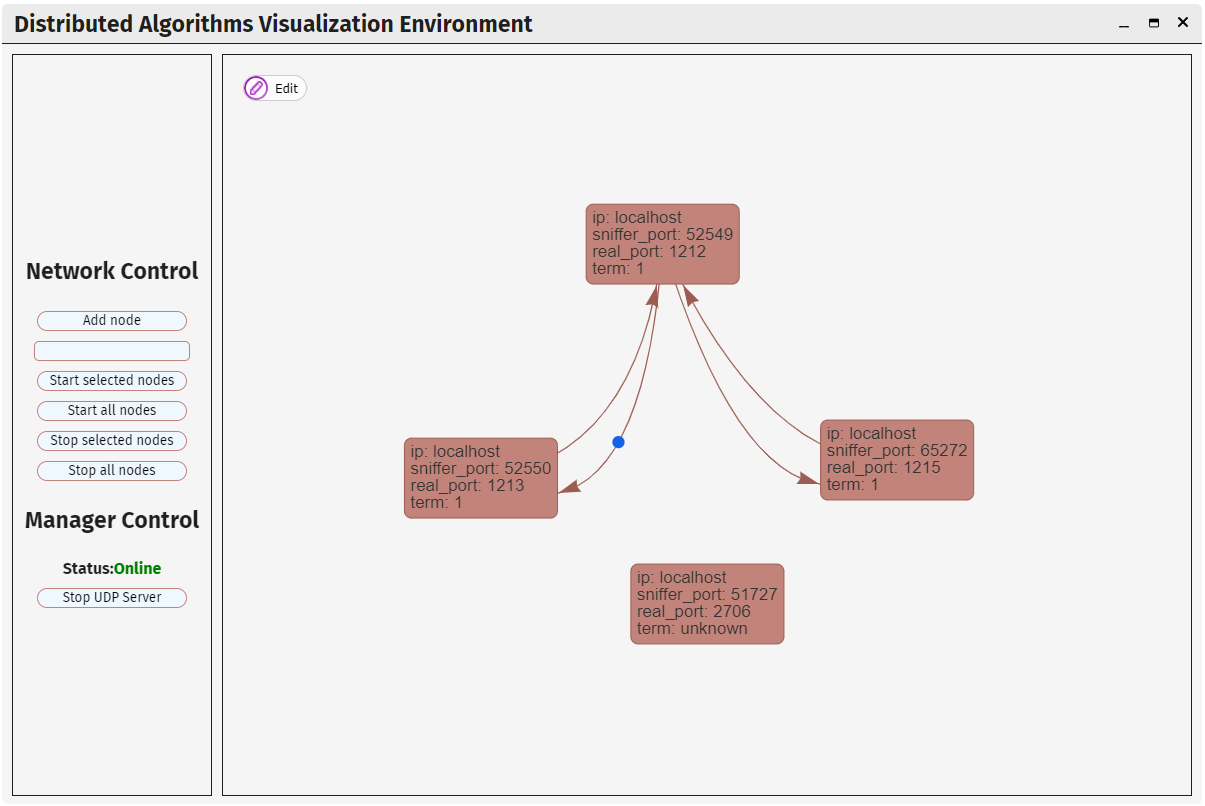
\includegraphics[width=0.9\linewidth]{imagenes/ui7}
\captionof{figure}{Añadir nodo nuevo durante la ejecución de otros nodos}
\label{fig:ui7}
}

%\begin{figure}[p]
%  \centering
%  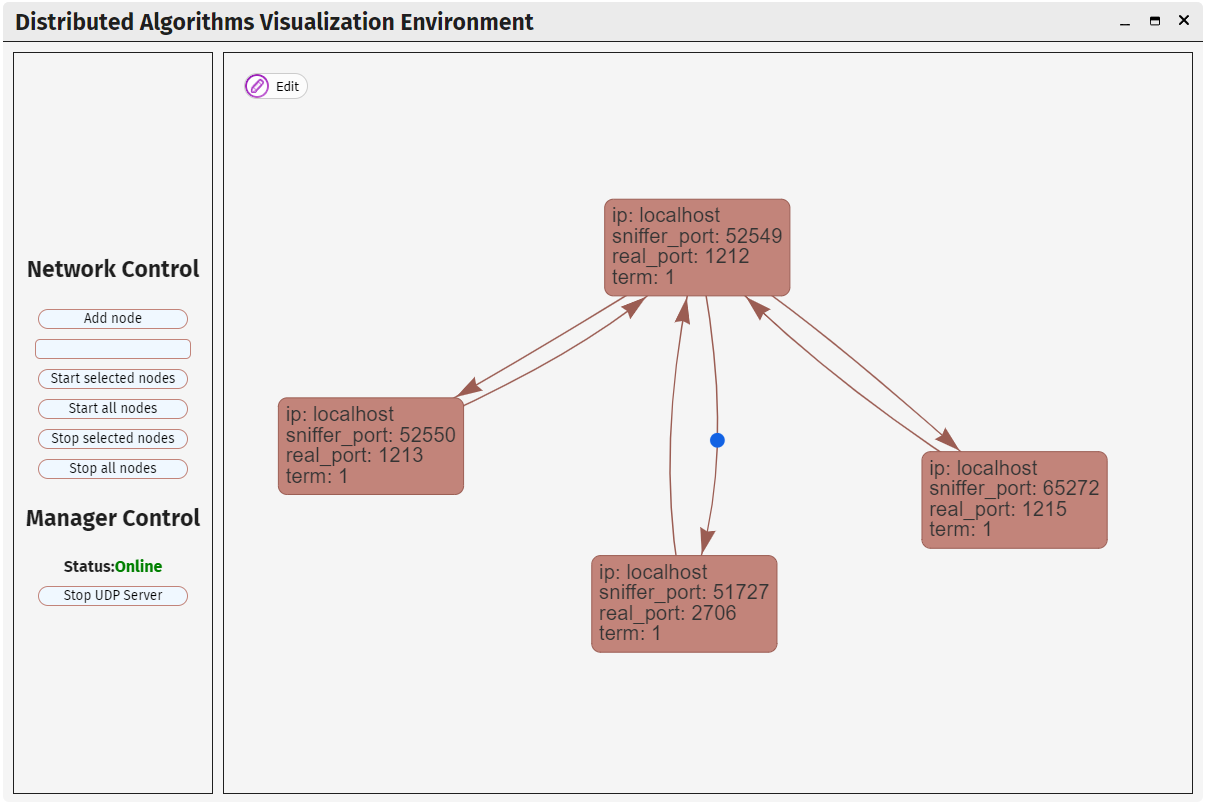
\includegraphics[width=0.9\linewidth]{imagenes/ui8}
%  \caption{Visualización del tránsito de mensajes con el nuevo %nodo}
%  \label{fig:ui8}
%\end{figure}
{
\centering
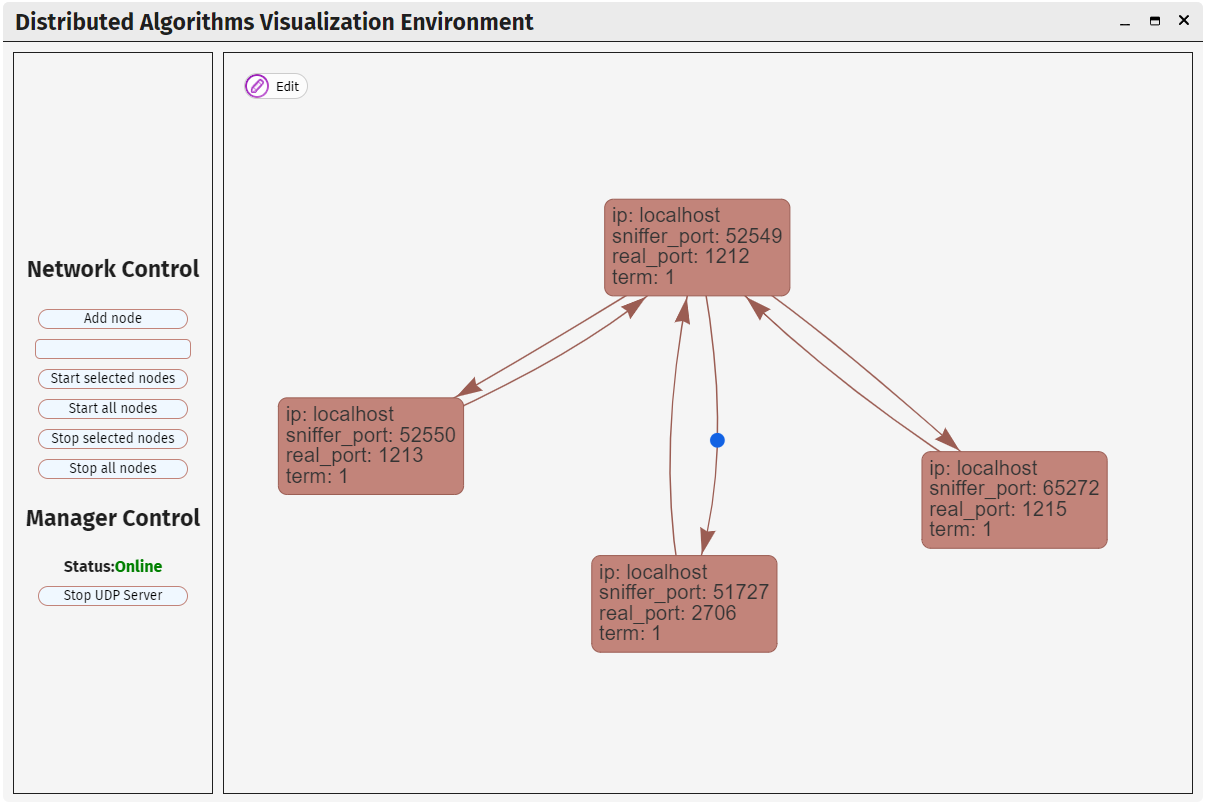
\includegraphics[width=0.9\linewidth]{imagenes/ui8}
\captionof{figure}{Visualización del tránsito de mensajes con el nuevo nodo}
\label{fig:ui8}
}

\newpage

\section{Comentarios sobre la implementación}

Como se ha descrito en la introducción, uno de los objetivos de este proyecto es proporcionar una herramienta que permita visualizar algoritmos distribuidos, permitiendo la posibilidad de intercambiar el algoritmo a visualizar. Tanto la arquitectura propuesta como la implementación permiten la visualización de otros algoritmos, sin embargo hay ciertos aspectos que es necesario tener en cuenta. No existe ningún formato universal de mensajes entre nodos de cualquier algoritmo distribuido, por tanto hay ciertos parámetros que se tienen que modificar para admitir el nuevo algoritmo.

\begin{itemize}
\item En primer lugar, se debe definir el formato de los mensajes para modificar debidamente las funcionalidades de la interfaz que muestran información sobre estos. Estas modificaciones se harían en el proceso \textit{manager}, dado que es el proceso que modifica la visualización del algoritmo.

\item También es necesario modificar el proceso capturador de tal manera que se comunica de la forma adecuada con el nuevo algoritmo. En el caso de esta implementación, el algoritmo se controla por la entrada estándar, pero podría darse el caso en el control se llevase a cabo desde un dispositivo o desde un \textit{socket}.
\end{itemize}

En lo restante de esta sección se comentarán tanto los requisitos para ejecutar el sistema, como las dependencias de cada módulo.

\subsection{Dependencias}

Para las máquinas que ejecuten el algoritmo, se requieren las siguientes dependencias:

\begin{itemize}
\item \textit{Go} - versión 1.17+. Para soportar la ejecución del algoritmo \textit{Raft}.
\item \textit{Python} - versión 3.9+. Para ejecutar el proceso capturador.
\item Sistema operativo: basado en \textit{Linux}. Esta restricción viene de que la función \texttt{sniffer} del proceso capturador requiere componentes de la librería \texttt{socket} de \textit{Python} que no están disponibles en otro tipo de sistemas operativos.
\end{itemize}

En cuanto a la ejecución de la interfaz, se requieren las siguientes dependencias:

\begin{itemize}
\item \textit{Node.js}.
\item \textit{electron}. Este paquete se puede instalar con el administrador de paquetes de \textit{Node.js}, con el mandato \texttt{npm install --save-dev electron}.
\end{itemize}

\newpage

\subsection{Ejecución del entorno}

La ejecución del entorno se divide en dos partes. Por una parte la ejecución de las instancias del proceso \textit{capturador}, y por  otra la ejecución de la aplicación de escritorio. Cada instancia del proceso capturador se inicia ejecutando el mandato \texttt{python sniffer.py} desde el directorio raíz del proyecto. La interfaz se puede ejecutar de dos formas: o bien desde el ejecutable generado por \textit{electron}, o con el mandato \texttt{npm run start} desde el directorio raíz de la implementación de la interfaz.
